\chapter{Background}

\section{Description of Fireballs}













\section{The D6 AllSky Camera}













\section{Photometry}





\subsection{Airplanes and other interference}







\section{Analysis}













\section{Existing Surveys}
While amateur astronomers and low-budget systems capture useful information, larger professional systems act as a vitally important comparison point.
Individual events captured by an observer do contribute to the pursuit of knowledge.
However, a small camera system that cannot yield similar data to more professional surveys serves only a marginal amount of utility.
Cameras for AllSky Meteor Surveillance (CAMS), the SPanish Meteor Network (SPMN), and the Lincoln Near Earth Asteroid Research (LINEAR) program are examples of well-established existing meteor observing surveys.  
All of these programs are continuously acquiring data and adding their findings to existing databases.  
Nearly all of this data is widely available, and is available to the public online. 



\subsection{CAMS}
Funded by NASA, Cameras for Allsky Meteor Surveillance (CAMS) aims to verify minor meteor showers and trace them back to their existing parent comets \cite{jenniskens_cams:_2011}.  
The project was created by Peter Jenniskens and is based in California.  
The CAMS network is spread across 3 different locations and consists of over 60 cameras.
By spreading their cameras across three separate locations, the CAMS research group can measure extremely precise trajectories of the incoming meteors. 
Similarly to the phenomena of trying to catch a baseball with only one eye open, confidently capturing a three dimensional trajectory of a fireball is extremely difficult when using only one camera.
Consisting of $3$ cameras located within $25$ miles of one another, as seen in Fig. \ref{trio} the CAMS survey have a median trajectory error of $0.31\deg$ and a median speed error of $0.53$ km/s \cite{jenniskens_cams:_2011}. 

\begin{figure}[ht!]
  \centering
  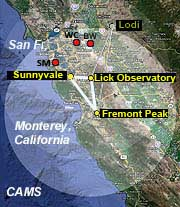
\includegraphics[scale=0.7]{images/CAMS_trio.jpg}
%   \setcaptioncitation{http://cams.seti.org/maps.html}
  \caption{The three CAMS network stations within a $50$ mile radius.}
  \label{trio}
\end{figure}

Accurate trajectories are particularly useful in back-tracing the motion of the meteor's orbit.  
The CAMS team has reduced over $320,000$ of these orbits \cite{seticams}. 
In addition to calculating orbits, CAMS also uses their precise velocity measurements to draw relations between speed and other properties. 
Figure \ref{fancyCAMS} shows the relationship between the apparent incident speed and peak magnitude.

\begin{figure}[ht!]
  \centering
  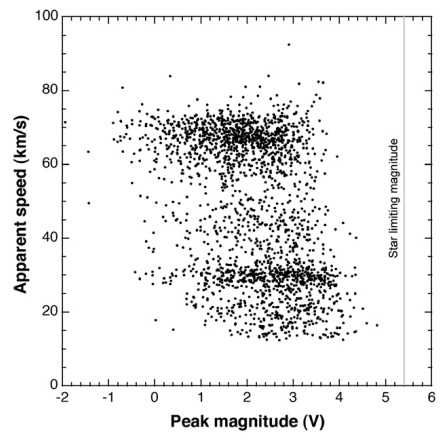
\includegraphics[scale=0.6]{images/CAMS_plot.png}
  \caption{Relationship between incident apparent speed and peak magnitude for CAMS data taken in November of 2010 \cite{jenniskens_cams:_2011}.}
  \label{fancyCAMS}
\end{figure}


Although the plot itself doesn't show a linear relationship, when considering the two subsets of relatively higher and lower incident speeds, we can see a general trend.
That trend shows that lower incident speed meteors tend to have slightly dimmer peak magnitudes. 



\subsection{SPMN}

The SPanish Meteor Network (SPMN) is 